%% ----------------------------------------------------------------
%% Hardware Development.tex
%% ---------------------------------------------------------------- 
\chapter{Initial Hardware and Firmware Development} \label{Chapter:HardwareDevelopment}
For initial development, the \textit{Il Matto} board, designed by Steve Gunn, which has an ATMega644P, was used. The system is clocked at 16MHz and has an on-board SD card connector. 

The following section is broken down into the following parts:
\begin{enumerate}
\item Camera Code
\item SD Card
%\item Motor Control
\item Circuit and PCB Development
\end{enumerate}

\section{Camera} \label{Section:Camera}

The camera used is an OV7670 by OmniVision. It is mounted onto a break out board and connected to a AL422B FIFO Buffer. The breakout board has all passive components needed and a 24MHz clock mounted. The schematic for the device can be seen in Appendix \ref{Chapter:AppendixA:CircuitDiagrams}.

Original code for the camera operation was given by Steve Gunn, of which I used to gain the operation required. The code streamed continuous video to a TFT screen. The operation required was to take a single photo. 

\subsection{Single Camera Operation}

The camera uses a SCCB Interface(\cite{SCCB_Interface}) created by OmniVision. This is almost identical to the $I^{2}C$ Interface by Phillips. The original code used a bit-banged SCCB interface which was very slow and used up processing time. This was changed to make used of the built in interrupt driven $I^{2}C$ interface (named TWI in Atmel AVRs)\footnote{$I^{2}C$ , SCCB and TWI are all the same but are called differently due to Phillips owning the right to the name ``$I^{2}C$"}. This communication bus is used to set up the control registers of the OV7670 to enable operation in the correct format. RGB565 is used in my application.

RGB565 is a 16 bit pixel representation where bits 0:4 represent the blue intensity, 5:10 is the green intensity and 11:15 represent the red intensity. This is a compact way of storing data but only allows 65536 colours. Greys can also appear to be slightly green due to an inconsistent colour ratio of the green field. 
\inote{figure to show this better?}
The camera must use a high speed clock in order to ensure the pixels obtained are from the same time. This makes it difficult for an AVRs (ATMegas typically clocked at 12-16MHz) to be able to respond to the camera quick enough. This highlights the importance of the necessity for a FIFO Buffer. 

The OV7670 is set up so that the VSYNC pin goes low at the beginning of every full frame of data and HREF is high when the data being output is valid. The pixel data is then clocked out on every rising edge of PCLK. To control the buffer, WEN (write enable) is NAND with the HREF signal. When both are high, the write enable to the buffer will be active and the data will be clocked in by PCLK. In order to acquire a full frame, the first VSYNC pin is set up to interrupt the AVR to enable WEN. The operation is then automatic and all the data is clocked into the buffer until the second interrupt of VSYNC where WEN is disabled. At this point, the entire frame of data is stored in the buffer.

To obtain the data from the buffer, the AVR sets output enable and manually pulses the read clock. Valid data is available on the input port chosen. All the data is then read in half a pixel at a time. 

Difficulties arose at this point with the storage of the data. The ATMega644P has 4kB of internal SRAM, but  153.6kB of memory is needed to store a single image at QVGA (320 by 240 pixels) quality. 

Firstly, data was sent straight to a desktop computer via a COM Port using USART. A simple desktop program was written in C\# to receive and store all the data, and to make a Bitmap image from the data. This method was slow, taking around 30 seconds to transmit one uncompressed image. 

The second option was to use extra memory connected to the microcontroller. An SD card was decided is used as FAT file system. This allows data to be looked at by a user on a computer. Text log files are also written to aid debugging. This is discussed in section \ref{sect:SDCard}. 
\inote{Put a figure of the pin timings in?}
\subsection{Dual Camera Operation}
In order for stereovision to be successful, two cameras separated by a horizontal distance, $B$, will need to be driven at the same time to obtain photos within a small time frame of one another.

The buffers have an output enable pin so the data bus can be shared by both cameras to the AVR. All buffer function pins are driven from pins, although a demultiplexer could be used if pins are short. The ATMega644P offers three interrupt pins, two of which are used by the two VSYNC pins for the cameras.

Two ISRs are used to control the VSYNC method and when taking a photo, both frames are taken at a time period close together to capture the same scenario. The data for both images are read back from one and then the other by the AVR. 

A major problem now occurred with using the \itc interface to set up both cameras. The camera has a set \itc address of $21_{16}$, which cannot be changed. Multiple \itc devices with exactly the same address cannot be used on the same bus. 
Two solutions to this are possible: driving one from $I^{2}C$ and one from SCCB, or using an \itc multiplexer. By using two different buses, there can be no bus contention. However, SCCB is slow and processor-hungry as it deals with the protocol bit by bit. Space for the code then has to be made and this code cannot be reused. 

An \itc multiplexer sits on the bus and has multiple output buses. The master can then address the multiplexer and select whether to pass the bus to bus 0, bus 1 or not allow the data to be transferred. This saves processor time, but means a write operation has to be done to select the camera bus before being able to write to the camera. This slows down the operation, but not as much as using SCCB. The main disadvantage to the \itc MUX is the extra hardware needed; firstly the MUX itself, but also 7 extra resistors to pull up the two extra buses and the three interrupt lines must be added. 

Overall, the disadvantages posed by using a MUX are small and simplify the operation and reduce the code size so an \itc MUX will be used. A suitable multiplexer is the Phillips PCA9542A (\cite{I2C_Mux}).

Operation to read an image is identical to using one camera. An ID number is passed through the functions to make a decision on the pins to use to read the buffer and to enable the output. Care was taken to avoid bus contention, but no checking procedure is explicitly in place. Both images are then read back from the buffers and stored to memory. 

\section{SD Card} \label{sect:SDCard}

To use the SD card, the FATFS library (\cite{FATFS}) was used. The library supplies all the functions for writing a FAT File System in the files \textit{ff.c}, \textit{ff.h}, \textit{ffconf.h}, \textit{diskio.c}, \textit{diskio.h} and \textit{integer.h}. The \textit{diskio.h} functions control what device is being used - SD/MMC Card, USB drive etc. The \textit{ff.h} header contains all the functions to write to in a FAT File system. 
\\
An SD card was chosen due to it's small size, low cost and a large data storage. The cards work using an SPI bus which can be used for other devices within the system so the card only uses one extra enable pin in hardware to function. 

\subsection{Storing Images}

Many image formats are common, such as Joint Photographic Expert Group (JPEG), Portable Network Graphics (PNG), Bitmap (BMP) and Graphics Interchange Format (GIF). Table \ref{ImageFormats} shows a summary of some common image formats.


\begin{table}
\centering
\begin{tabular}{|p{3cm}| p{3cm}|p{3cm}|p{3cm}|p{3cm}|} \hline
			&	Bitmap 		& 	JPEG			 	&	PNG				& 	GIF \\ \hline
Extension 		& 	*.bmp 		&  	*.jpg /*.jpeg 		& 	*.png				& 	*.gif \\ \hline
Compression 	& 	No 			& 	Lossless  and Lossy		&	Lossless ZIP			&	Lossy	\\\hline
File Size of 320 by 
240 pixel Image (kB) &	225			&	20				&	23				&	24 \\\hline
Bits per Pixel		&	8, 16, 24 or 32	&	24				&	24, 32 or 48 			& 	24, but only 256 Colours \\


\hline
\end{tabular}
\caption{A table comparing different image formats available (\cite{ImageComparison})}
\label{ImageFormats}
\end{table}

It is clear that the best choice for images would be either PNG or JPEG. However, these require much computational time to compress the image into the correct format. To avoid compression, and thereby save processing time, bitmap was chosen at the expense of using more memory. The data in a bitmap image is also stored in RGB format so can be read back easily when processing the data. Appendix \ref{Chapter:AppendixB:BMPFile} shows the make up of a Bitmap File that was used.

By writing the image in this format, the images are then able to be opened on any operating system. This aids debugging and allows the protoyping of image algorithms in a more powerful environment. Figure \ref{ExampleImage} shows a photo taken by the OV7670 and stored on a SD card.

\begin{figure}
\begin{center}
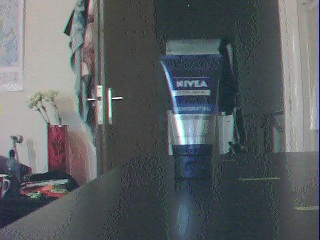
\includegraphics{Figures/ExampleImageFromCamera.jpg} 
\end{center}
\caption{An Example Image taken using the OV7670 and stored as a Bitmap on the SD Card}
\label{ExampleImage}
\end{figure}

\subsection{User Interface}
The ATMega 664P pinout for the dual camera operation can be seen in table \ref{table:644Pin}. Due to a lack of available GPIO pins, an ATMega 168 was added on the \itc bus to act as a port extender. The ATMega168 accepts a read or write, places the written data on Port D and reads in the lower nibble of Port C. When a button is pressed, this is stored in the ATMega168 until a read has been done. This is so the master (644P) does not miss any button presses while busy doing lengthy operations such as writing an image. The code is based on \cite{Atmel:I2CSlave}, written for IAR Compiler. This code was altered to compile with GCC under Atmel Studio. AVRs contain a hardware based \itc protocol that is interrupt based in software. The interrupt service routine of the TWI vector is a state machine which loads the data to send, stores received data, responds to acknowledges and address calls and deals with bus errors that can occur.

\begin{table}
\centering
\begin{tabular}{|c|c|c|c|c|}\hline
	& 	Port A 	& 	Port B 			& 	Port C 				& 	Port D 		\\ \hline
0	&	Data 0	&	SD Write Protect&	\itc - SCL			&	No Connection	\\
1	&	Data 1	&	SD Card Detect	&	\itc - SDA			&	No Connection	\\
2	&	Data 2	&	USB Data Plus	&	Read Clock 1		&	VSync 0			\\
3	&	Data 3	&	USB Data Minus	&	Read Reset 1		&	VSync 1			\\
4	&	Data 4	&	SPI Chip Select	&	Write Enable 1		&	Read Clock 0	\\
5	&	Data 5	&	SPI	MOSI 		&	Write Reset 1		&	Read Reset 0	\\
6	&	Data 6	&	SPI MISO		&	Output Enable 0		&	Write Enable 0	\\
7	&	Data 7	&	SPI Clock		&	Output Enable 1		&	Write Reset 0	\\
\hline

\end{tabular}
\caption{Pin Connections of the ATMega 644P for Dual Camera Operation.}
\label{table:644Pin}
\end{table}
%\section{Motor Control}
%\inote{do something of this SOON}
\section{Circuit and PCB Development}
\subsection{Il Matto Development}
Figure \ref{sch:DualCam_Schematic} shows the circuit diagram for the prototype. This uses the Il Matto development board for the main microcontroller. The prototype can be seen in figure \ref{fig:Prototype}. 

\begin{figure}
\includegraphics[width=\textwidth]{./Figures/Prototype.jpg}
\caption{Prototype of Dual Camera operation.}
\label{fig:Prototype}
\end{figure}